\documentclass[letterpaper, 10 pt]{sig-alternate-10pt}
\usepackage{graphics}
\usepackage{graphicx}
\usepackage{subfigure}
\usepackage{epsfig}
\usepackage{url}
\usepackage{balance}
\usepackage{amsmath}
\usepackage{helvet}
%\usepackage{verbatim}
%\usepackage{amsfonts}
%\usepackage{amssymb}
%\usepackage{amsthm}


% MATH -------------------------------------------------------------------
\newtheorem{thm}{Theorem}[section]
\newtheorem{prop}{Proposition}
\newtheorem{lem}{Lemma}
\newtheorem{cor}{Corollary}

\newif{\ifanonymous}
\anonymousfalse
%\anonymoustrue
\newcommand{\appsection}[1]{\let\oldthesection\thesection
  \renewcommand{\thesection}{Appendix \oldthesection}
  \section{#1}\let\thesection\oldthesection}

\newcommand{\comment}[1]{}
\newcommand{\smallcaption}[1]{\caption[#1]{{\protect\small \protect\bf #1}}}
\newcommand{\fakeitem}{\vspace*{1ex} \noindent $\bullet$ \hskip .02in}


\begin{document}

\title{{LANCOM}:A Language for Security and Routing Information Management and Configuration}

%\ifanonymous
%\numberofauthors{1}
%\author{Anonymous submission to ACM SIGCOMM/USENIX IMC 2007 \\}
%\else
%\numberofauthors{1}
\author{
\alignauthor {Ashish S Tomar, Chitra S Agastya, Milind Nimesh,Nipun Arora and Sambuddho Chakravarty}\\ 
\affaddr {Dept.of Computer Science, Columbia University}\\
\affaddr {New York, NY}	\\
\email {\{ast2124,csa2111,mn2353,na2271,sc2516\}}@columbia.edu\\
}
%\fi

\maketitle

\section{Introduction}
\label{sec:introduction}

Misconfiguration of security and networking devices is a source of
  vulnerabilities for various commercial and private network.
  System administrators cannot be solely be held responsible for such
  misconfiguration. Commercial networking and security device manufacturers have their own
  syntax for management and configuration. Some, such as CISCO IOS,
  have become de facto standards which are `` adhered to '' by other vendors.
  However, broadly speaking, there is no standard syntax for router and 
  firewall configuration.   This complicates the configuration tasks for system administrators,
  who deploy such devices in large corporates.The system administrator (s) need to be
  familiar with the language peculiarities of various   configuration interfaces, increasing 
  the chances of misconfiguration and introducing redundant and ineffective routing and firewalling
  policies. A common vulnerabilty in firewalling configuration arises due to the order in which the 
  semantic analyzer analyzes the rules. Firewall configurations may be as simple 
  as packet filtering rules; maybe much more complex such for stateful firewalling,
  protocol specific vulnerability detection and deep packet inspection.
  Certain firewalls match the incoming packets to the first matched rule
  while the others match the last one.The absence of any particular firewall and router configuration
  language motivates us to design {\bf LANCOM} ({\bf LA}nguage for {\bf N}etwork {\bf CO}nfiguration and
  {\bf M}anagement). We plan to design, implement and test LANCOM with the following objectives:

  \begin{enumerate}
    \item `` Device manufacturer independent '' description of firewalling and
             routing configuration. 
    \item  Separation between network topology and
           firewalling policy description.We intend to achieve this using 
           {\it role - based} policy description. 
  \end{enumerate}

Following figure ~ \ref {fig:block_dgm} presents a rudimentary description of 
the language compiler can and how it can be used to generate vendor specific 
 routing and firewalling configuration scripts. 

\begin{figure}[ht] 
\label {fig:block_dgm}

%\centering 
\begin{center}
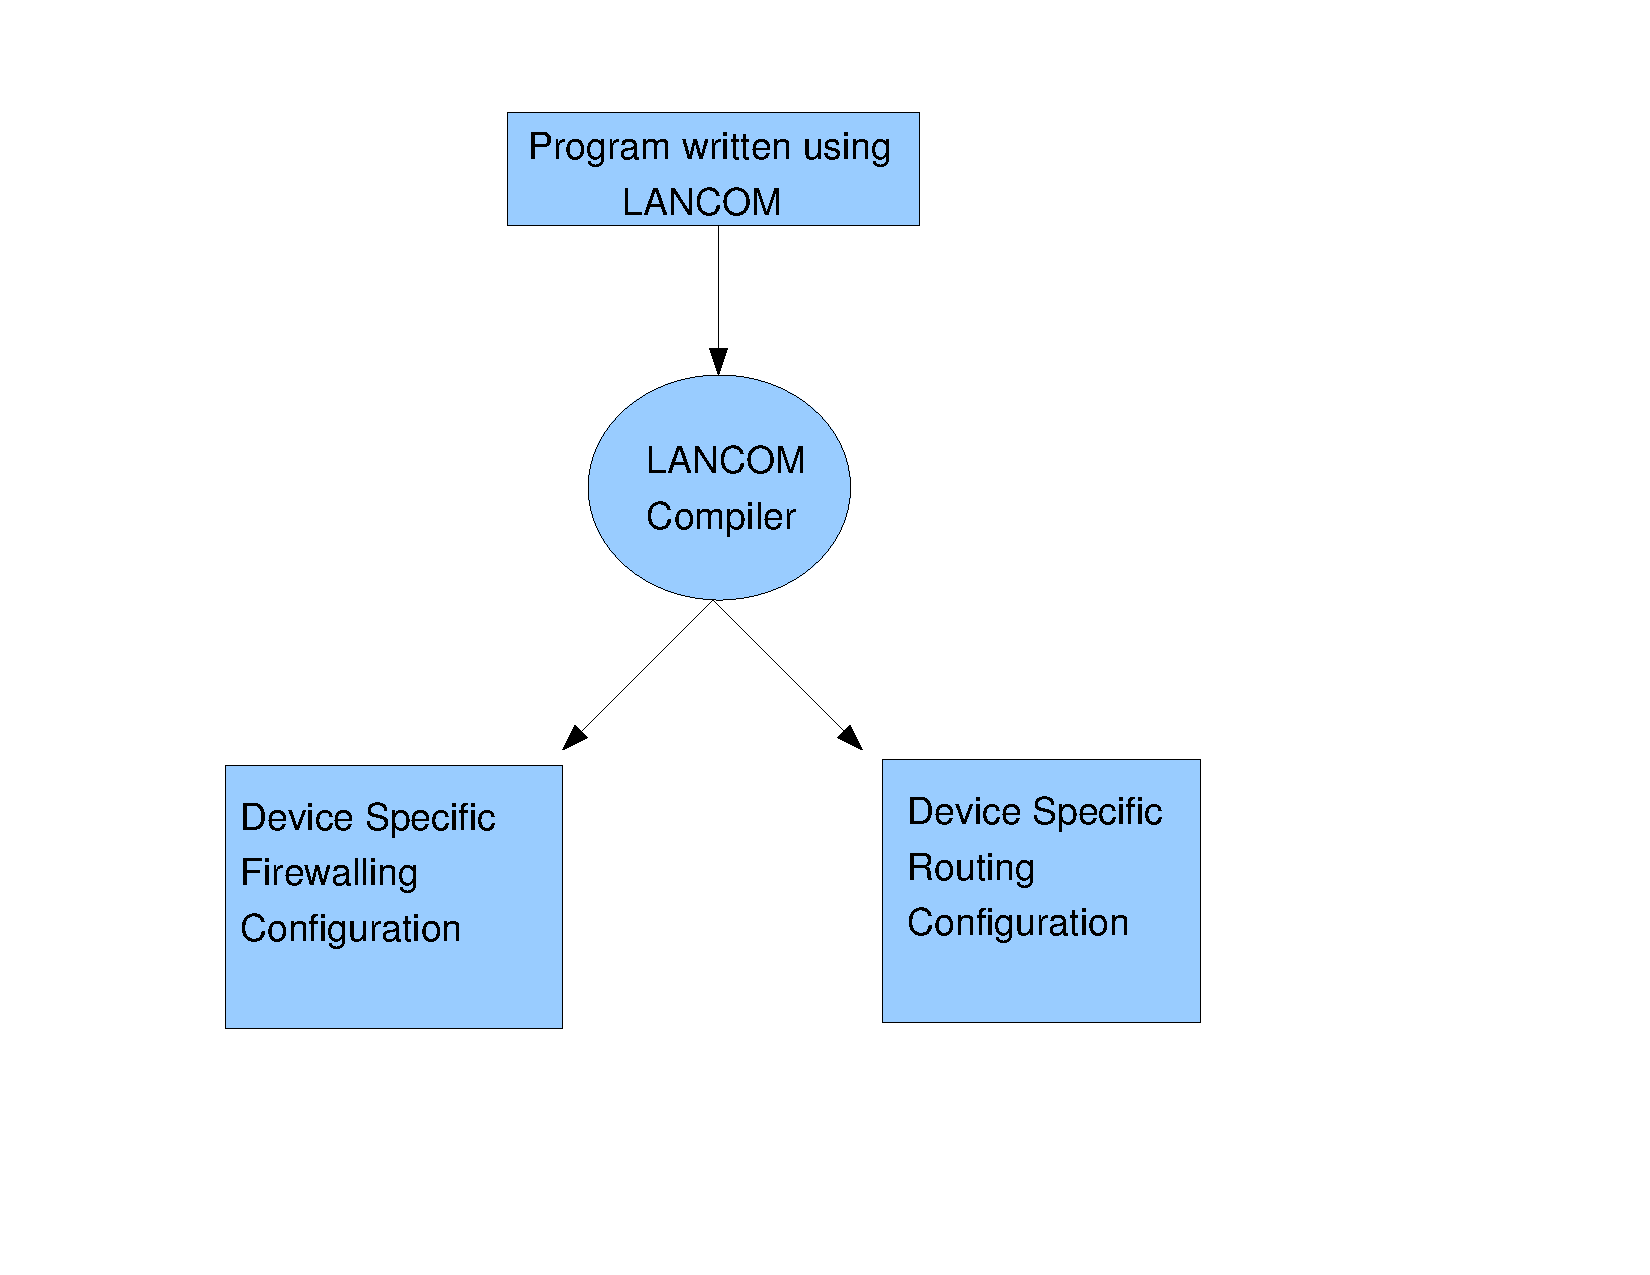
\includegraphics[scale=0.35]{figs/language_blk_dgm.pdf}
\end{center}
\smallcaption {The LANCOM Compiler Generates Output Specific to the Firewall / Router}
 \end{figure}

\section{Related Work}
 \label{sec:related_work}

We next describe in brief, some research work relevant to our efforts.
  We being with describing a language called Firmato and conclude with the
  efforts presented by S.Ioannidis as a part of his doctoral thesis. 
  Firmato \cite{bartal99firmato} is perhaps the most relevant research in the area 
  of machine independent security policy description languages.  The objective of 
  Firmato is device independent security policy description.Secuity policies are 
  described in terms of objects with characteristics and properties.Further these 
  objects may be grouped into sets. These sets may be specified in the form of 
  `${\tt host\_group}$' and `${\tt service\_group}$'. A `${\tt host\_group}$ '
    is a set of hosts (say possibly within the same subnet. Fimato relies heavily 
  on attribute and property inheritance/seperation (for objects belong to the set contaning it). 
  This is achieved through a concept of $CLOSED$ and $OPEN$ addition to sets. When a new `${\tt host}$' 
  object is added to the group it inherits the properties of the set by default (addition to a set is $OPEN$ by default).
  However, when addition is explicity $CLOSED$, the object doesn 't inherit the security policies of the set.

Another research, closely relevant with our efforts, uses Lisp like language definition for 
defining packet filtering policies \cite{guttmanfiltering}. The language consists of notations
 for representing network specification, services and policies.  The authors however don't
 clarify how it can be used to generate firewall rules.

We conclude this section with a very relevant work done by S.Ioannidis \cite{ioannidis}.
The author addresses issues related to securing heterogenous and complex computer networks.
The dissertation discusses complexities arising from various network elements and the 
topologies through high level security and access control policy description.
The dissertaion highlights enforcing organizational level security policies
through automated and semi-automated tasks. 

Through LANCOM we try to provide an out of the box solution to the problem of seucrity policy and network topology 
description. An administrator of a complex network may use LANCOM to configure an array of routers and firewalls effortlessly.

\section{Language Buzzwords}
\label{sec:buzzwords}

Through our prototype of LANCOM we intend to demonstrate a common high -
  level language for router and firewalling configuration.Particularly,
  we attempt to design a language which maintains separation of network
  topology and routing information description from firewalling and security
  policies.Using role based access control \cite{bartal99firmato}
 , we intend to configure any policy on any routing and networking topology
  description with minimal modifications. We borrow the concept of encapsulation
   from object oriented programming to describing the network entities and roles as objects.
  These objects are collection of attributes and methods. Attributes of the objects of classes
   describing policies and roles maybe used to act upon attributes of objects of 
  classes describing networking topology.

\begin{itemize} 
 
 \item \noindent {\bf Ease of use}: Commercial routers and firewalls have 
    their own syntax constructs and peculiarities. A system administrator 
    needs to expend time and effort in in learning such syntices.A small sized 
    networks may deploy devices from various vendors. Configuring all such devices,
    keeping in mind the syntactic and semantic peculiarities of the
    configuration languages of all these devices, adds up to the ever increasing 
    and daunting responsibilities of the human
    administrator. 

 \begin{figure}[ht] 
 \label{fig:ease_of_use}
  %\centering 
 \begin{center}
  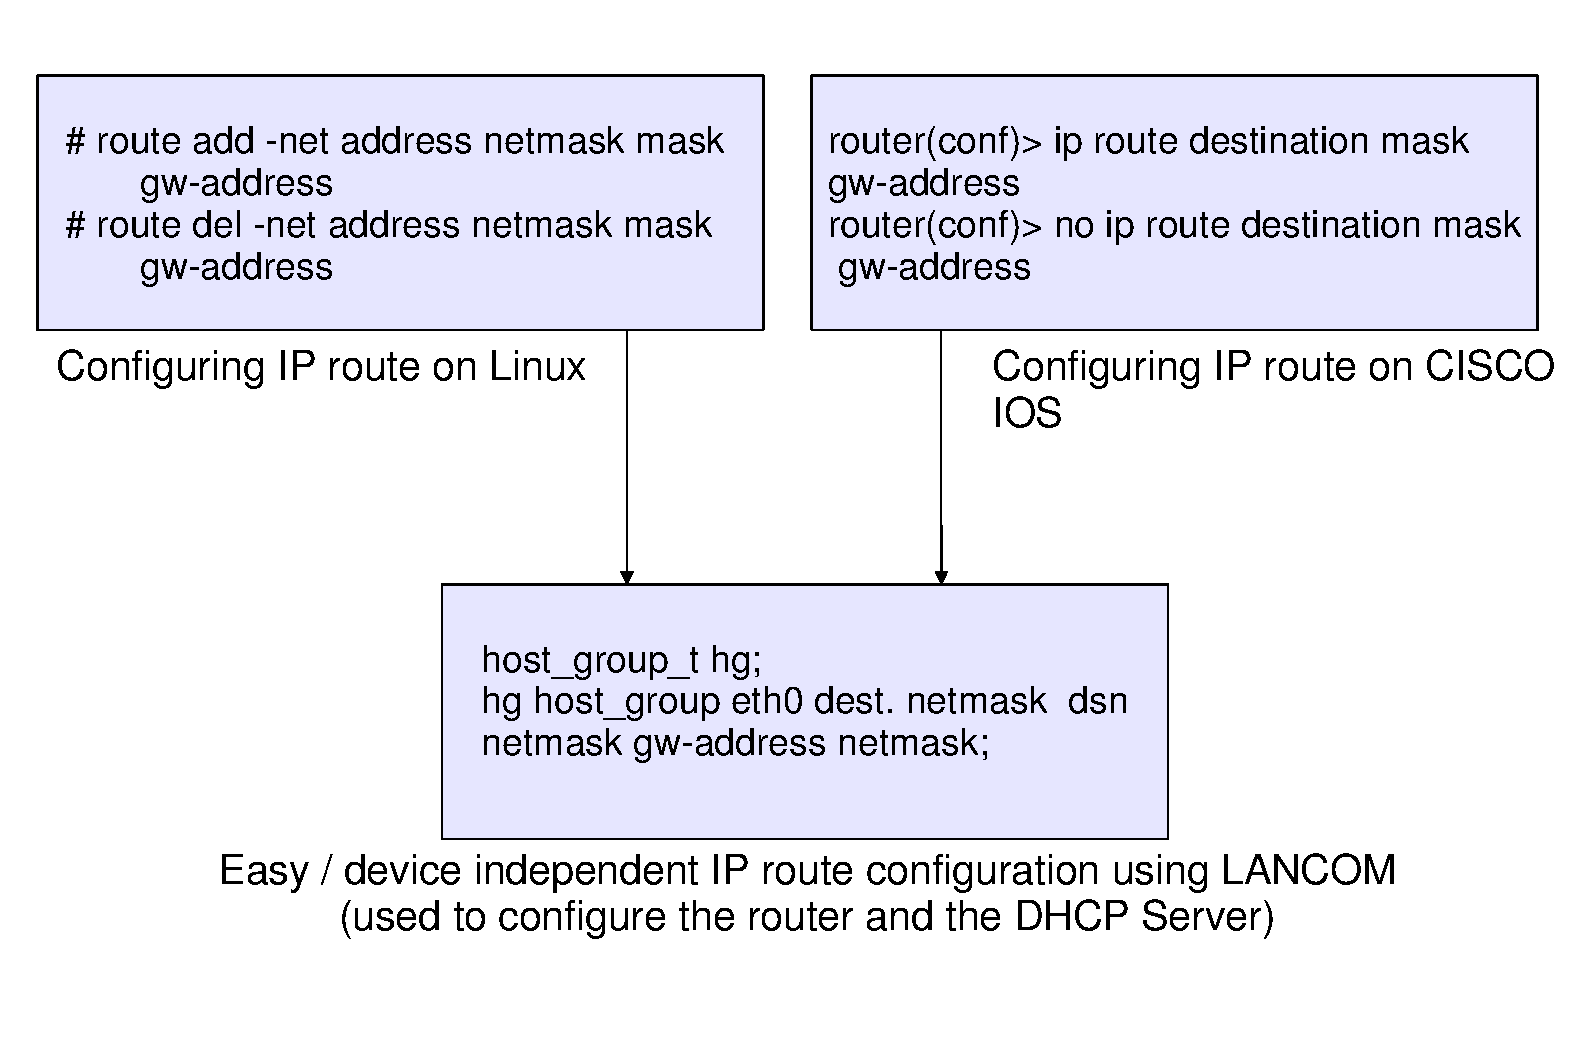
\includegraphics[scale=0.35]{figs/ease_of_conf.pdf}
  \end{center}
  \smallcaption{LANCOM makes it easy for a system administrator to write device
      independent routing and firewalling configurations}
   \end{figure}

   

%Let us take the example of a small network of linux PCs connected with a
%Cisco router and ethernet hubs. n order to statically configure a routing table,
%the user needs to f %
%amiliarize himself with the routing commands on linux OS as well as the
%routing command on Cisco 's IOS. And these sets of commands are different. Imagine the complexity of co% nfiguring a network with several hundreds of PCs running different operating systems and supporting different routers! 

Through LANCOM, we aim at relieving administrators the responsibility of learning the configuration syntices of the various routing and firewalling devices his organization uses. It aims to be a common language, that can be used to configure any interface or firewall in the network. Figure ~\ref{fig:ease_of_use} shows how LANCOM can be replaced by multi-lingual configutation syntices. This saves the user the time and effort needed to learn multiple commands on different systems and allows them to focus on configuring topologies and designing security policies.

\item \noindent {\bf Portability}: We aim at providing a common high-level interface across multiple systems. It enables unified management of networking elements from different vendors/manufacturers. It may ideally ease the transition of an organization' s switching networking products from one vendor to another. 

\item \noindent {\bf Flexibility}: We propose separation between security policy description from the
	network topology description. We aim to provide the users with flexibility of configuring firewalls,
	``independent '' of specifying the networking topology and routing
	information. Moreover, the very nature of the grammar being relatively ``small'',
	promises modularity and granularity. 

\item \noindent {\bf Scalability}: LANCOM would scale across various network sizes.
      Since we propose a relatively ``small'' but robust grammar,
      LANCOM maybe used for describing the network topology, routing information and security policy,
      {\bf regardless of the number of devices attached}. The language shall not impose restrictions on 
      the magnitude of the network. 

\begin{figure}[ht] 
\label{fig:scalability}
    %\centering 
\begin{center}

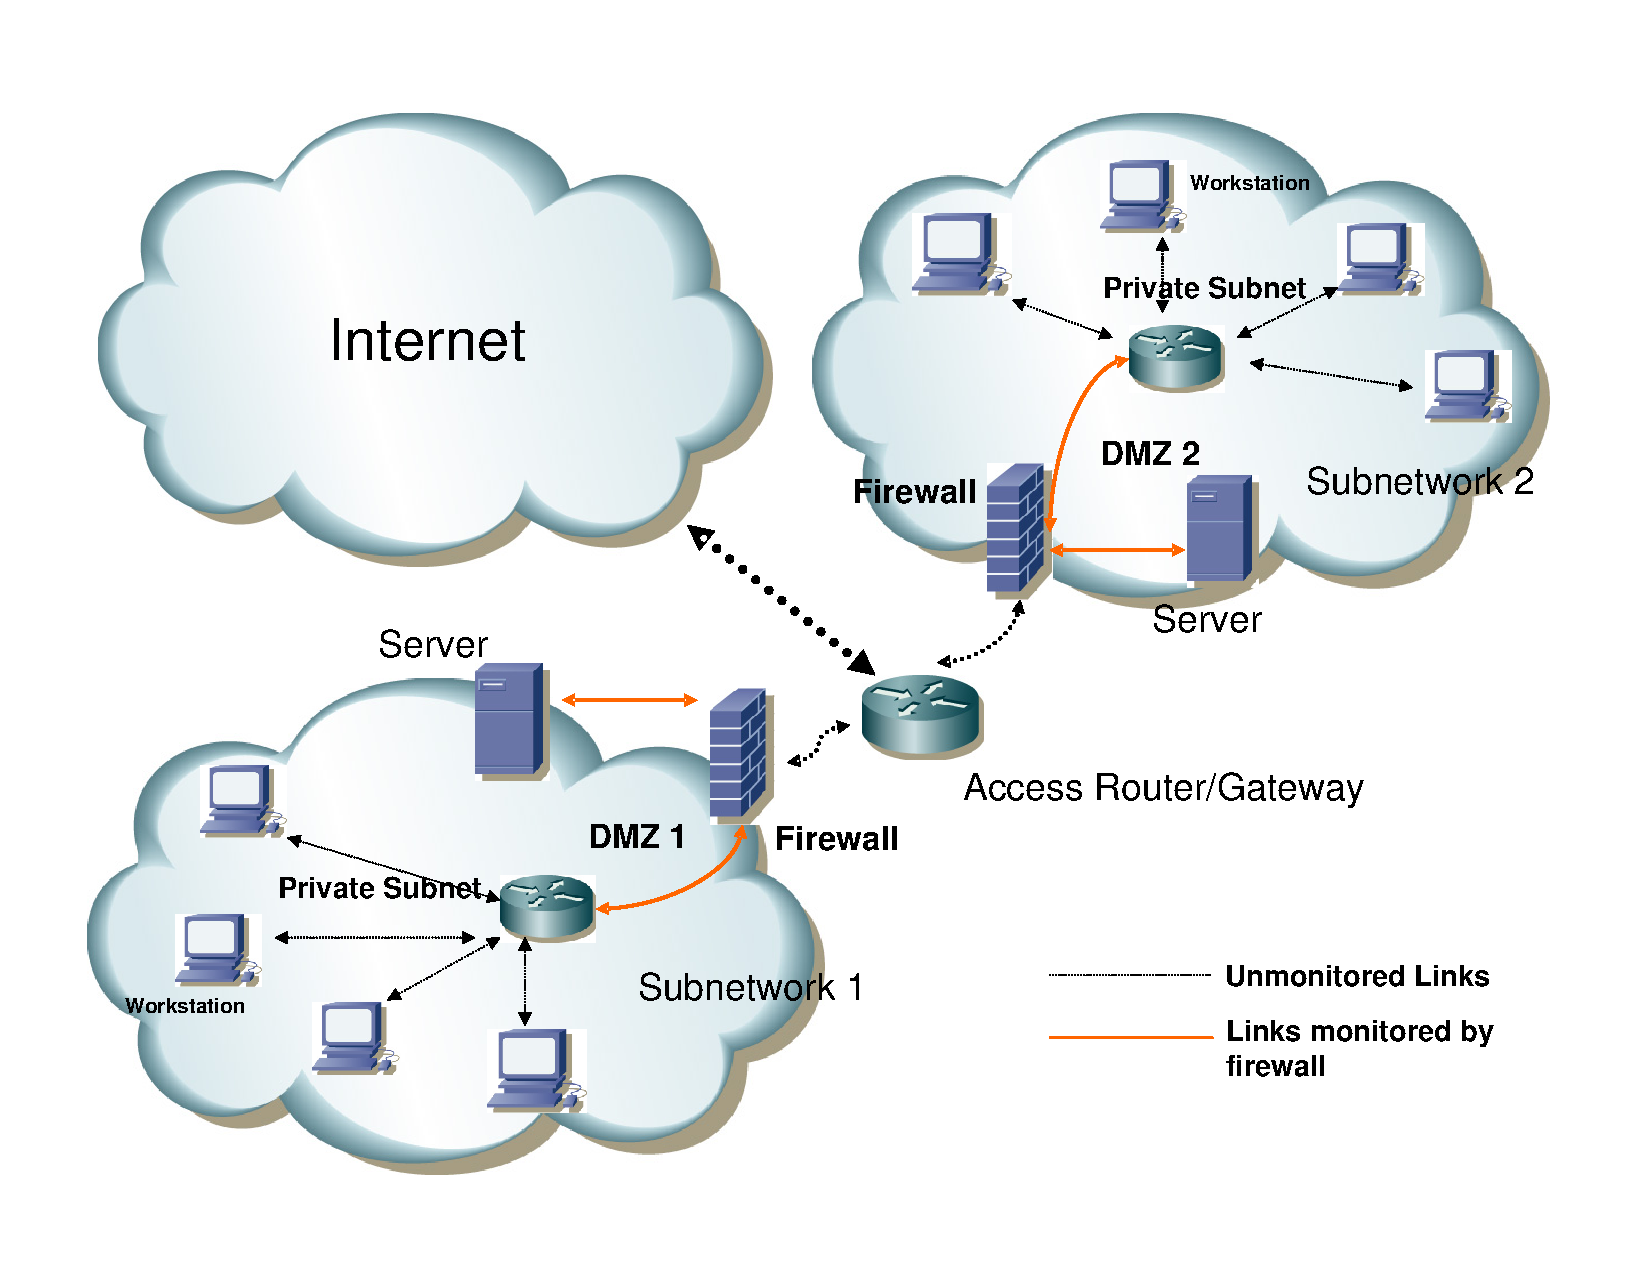
\includegraphics[scale=0.3]{figs/scalability.pdf}
\end{center}
\smallcaption {LANCOM may make configuration independent on the size of the network and
	the underlying toplogy}
\end  {figure}
     %Our language is mainly intended to be used by the System Administrators or in the field of System and Security 
%   Management for configuring routers and firewalls in a large company setup.In such a scenario Scalability will play a very important 
%  role as there can be a large set of inter connected systems on a network overlay.Our language can be used to configure � �n � �number 
%  of computers and routers simultaneously and hence reducing the overhead involved.The language will not impose any restrictions on the 
%  size of the network and will be scalable to accommodate networks as they grow larger or smaller. 


\item \noindent {\bf Reliability}: The LANCOM compiler shall produce configuration files that can be used
	  directly to configure systems.We hope to produce, to the best of our knowledge and abilities,
	  parsers and semantic analyzers which would generate configurations
	  free from security bugs and misconfiguration. 




\item \noindent{\bf Re-usability}: The final, and maybe the most important reason for us
	to design LANCOM, is to reduce the workload and overhead involvedn
          in configuring various firewalls and routers.We plan to add re-usabilty 
          to the language through constructs such as macros and
	  procedure calls.

 \end{itemize}

That said, we show give an overview of grammar used by LANCOM and how it can be used 
by administrators to generate configuration, without knowledge of the vendor specific language syntax.

\section {Some Sample Grammatical Constructs / Snippets of LANCOM}
 \label {sec:grammatical_snippets}

This section presents how the language constructs ``look'' like.
  The language constructs of LANCOM are quite similar to Firmato.
  The grammar for LANCOM would dictate how network entities and firewalling
  policies be represented using a device independent language.
  A key goal of our language is clear separation of firewalling policy
  description and topology description.
  Such a separation allows an administrator to independently describe routing
  and firewalling configurations.
  The next subsection shows exactly how this is achieved. 

\subsection{Some Sample Grammatical Constructs}

In this subsection,
  we present some of the grammatical constructs of LANCOM.As of now,
  we limit the capabilities of the language to simply represent configuration
  in the form of topology and role based representation.
  Later we shall expand the language to include conditional and looping
  constructs. \\ 

\begin{enumerate}
 \item \noindent ${\it statement}$ $\rightarrow$ ${\it expression}$ $({\it statement})^{*}$ ${\it delimiter}$ \\ 
  \item ${\it expression}$ $\rightarrow$ ${\it type\_name}$ ${\it object\_name}$ \\ 
  \item ${\it expression}$ $\rightarrow$ ${\it object\_name}$ ${\it attrib}$ ${\it attrib\_values}$ \\\\ 
  
\item \noindent ${\it attrib}$ $\rightarrow$ ${\tt topology}$ \\ 
\item ${\it attrib}$ $\rightarrow$ ${\tt host\_group}$ \\
 \item ${\it attrib}$ $\rightarrow$ ${\tt host}$ \\ 
\item ${\it attrib}$ $\rightarrow$ ${\tt service\_group}$ \\ 
\item ${\it attrib}$ $\rightarrow$ ${\tt role}$ \\ 
\item ${\it attrib}$ $\rightarrow$ ${\tt policy}$ \\\\ 


\item \noindent ${\it attrib\_values}$ $\rightarrow$ ${\it topology}$ \\ 
\item ${\it attrib\_values}$ $\rightarrow$ ${\it host\_group}$ \\ 
\item ${\it attrib\_values}$ $\rightarrow$ ${\it host}$ \\ 
\item ${\it attrib\_values}$ $\rightarrow$ ${\it service}$ \\ 
\item ${\it attrib\_values}$ $\rightarrow$ ${\it service\_group}$ \\ 
\item ${\it attrib\_values}$ $\rightarrow$ ${\it role}$ \\ 
\item ${\it attrib\_values}$ $\ rightarrow$ ${\it policy}$ \\\\ 

\item \noindent ${\it type}$ $\rightarrow$ ${\tt topology\_type\_t}$ \\ 
\item ${\it type}$ $\rightarrow$ ${\tt host\_type\_t}$ \\ 
\item ${\it type}$ $\rightarrow$ ${\tt host\_group\_type\_t}$ \\ 
\item ${\it type}$ $\rightarrow$ ${\tt service\_group\_type\_t}$ \\ 
\item ${\it type}$ $\rightarrow$ ${\tt role\_type\_t}$ \\ 
\item ${\it type}$ $\rightarrow$ ${\tt policy\_t}$ \\ 
\item ${\it object\_name}$ $\rightarrow$ $[{\tt 0-9,a-z,A-Z}]^{+}$ \\\\ 

\item \noindent ${\it delimiter}$ $\rightarrow$ ${\tt;}$ \\ 

\item \noindent ${\it topology}$ $\rightarrow$ $({\it host\_group})^{*}$ $({\it role})^{*}$ \\ 
\item ${\it topology}$ $\rightarrow$ $({\it service\_group})^{*}$ $({\it role})^{*}$ \\ 
\item ${\it host\_groups}$ $\rightarrow$ $({\it host})^{+}$ $({\it dns})^{*}$ $({\it def\_gw})^{*}$ \\
\item ${\it dns}$ $\rightarrow$ ${\it host}$ \\ 
\item ${\it def\_gw}$ $\rightarrow$ ${\it host}$ \\ 
\item ${\it host}$ $\rightarrow$ (${\it interface\_name}$) (?) ${\it ip\_addr}$ ${\it netmask}$ \\ 
\item ${\it netmask}$ $\rightarrow$ ${\it ip\_addr}$ \\ 
\item ${\it interface\_name}$ $\rightarrow$ $[{\tt 0 - 9, a - z, A - Z}]^{+}$ \\ 
\item ${\it ip\_addr}$ $\rightarrow$ {\tt [0-255]}.{\tt [0-255]}.{\tt [0-255]}.{\tt [0-255]}\\
\item ${\it service\_group}$ $\rightarrow$ ${\it ip\_addr}$ ${\it netmask}$ ${\it serv\_listen\_port}$ \\ 
\item ${\it serv\_listen\_port}$ $\rightarrow$ {\tt [0-65536]}\\\\

\item \noindent ${\it role}$ $\rightarrow$ $({\it policy})^{*}$ \\
\item ${\it policy}$ $\rightarrow$ ${\it direction}$ ${\it verdict}$ ${proto}$ ${\it port}$ ${\it port}$ \\ 
\item ${\it policy}$ $\rightarrow$ ${\it direction}$ ${\it verdict}$ ${\it icmp\_cntrl\_message}$ \\ 
\item ${\it direction}$ $\rightarrow$ ${\tt inbound}$ \\ 
\item ${\it direction}$ $\rightarrow$ ${\tt outbound}$ \\ 
\item ${\it verdict}$ $\rightarrow$ $({\tt allow}|{\tt deny})$ \\ 
\item ${\it proto}$ $\rightarrow$ ({\tt UDP $ | $ TCP}) \\ 
\item ${\it icmp\_cntrl\_message}$ $\rightarrow$ ({\tt ICMP\_MESSAGE\_TYPE}) \\ 
\item ${\it port}$ $\rightarrow$ {\tt [0-65535]}\\
\end{enumerate}

  Clear seperation of routing information and firewalling policy description
  is evident from the seperation of rules for both both tasks.
   For the sake of testing, we choose the back - end for LANCOM as Linux
  {\it iptables} or FreeBSD {\it pfilter}. However, the flexibility of LANCOM 
   shall allow any administrator to specify configuration, independent of the 
   vendor specific syntax. A sample program in the next subsection shows how
  the language may be translated into Linux routing and firewalling commands.

 \subsection{Sample Program Snippet Using LANCOM}

  We next show a small example program written using LANCOM and a possible
  equivalent translation to Linux routing and 'iptables' firewalling
  configuration. \\

 \noindent \{\\
  \indent ${\tt topology\_t}$ $tp$;\\
  \indent ${\tt host\_group\_t}$ $hg$;\\
  \indent ${\tt service\_group\_t}$ $sg$;\\
  \indent ${\tt hg}$ ${\tt host\_group}$ ${\tt eth0}$ $128.59.0.0$ $255.255.0.0$ $128.59.16.20$ $255.255.255.255$
          $128.59.16.1$ $255.255.255.255$;\\

  \indent ${\tt role\_group\_t}$ $rg$;\\
  \indent ${\tt policy\_t}$ $pl$;\\
  \indent ${pl}$ ${\tt policy}$ ${\tt inbound}$ ${\tt TCP}$ ${\tt allow}$ $80$ ${\tt any}$;\\
  \indent ${rg}$ ${\tt role\_group}$ $pl$;\\
  \indent ${sg}$ ${\tt service\_group}$ $128.59.23.168$ $255.255.255.255$ $80$;\\
  \indent ${tp}$ ${\tt host\_group}$ $hg$;\\
  \indent ${tp}$ ${\tt service\_group}$ $sg$ $rg$;\\

\}


    The first line of the program begins by declaring an object of type ${\tt topology\_t}$.
    As per LANCOM grammar it is a collection of attributes which are objects of other types such 
    as ${\tt host\_group\_t}$. The attributes of ${\tt hg}$, ${\tt host\_group}$ is expanded from
    the rule $27$. It specifies the IP address of the subnet connected to network interface
    ${\tt eth0}$, the DNS server address and the default gateway. The ${\tt role\_group\_t}$ 
    object $rg$, is defined to contain policy $pl$. The policy $pl$ is to be translated to a 
    firewalling rule which should allow inbound connections to $TCP$ port $80$.The ${\tt service\_group}$
    object ${\tt sg}$ represents a web server waiting for incoming connection on IP 
    address $128.59.23.168$ and port $80$.

    The following is the equivalent routing configuration which results from
    compilation of the above program.\\ 

\noindent ${\tt route}$ ${\tt add}$ ${\tt -net}$ $128.59.0.0/16$ ${\tt dev}$ ${\tt eth0}$ \\

    All packets with destination IP address in subnet $128.59.0.0/16$ would be sent out of 
    network interface ${\tt eth0}$. For each host belonging to the subnet, the DNS server and
    default gateway would be $128.59.16.20$ and $128.59.16.1$ respectively. This information 
    may be used within the ${\tt DHCP} $ server process of the router and may be send to clients 
    through ${\tt DHCP}$ ${\tt offer}$ messages.

    The following are the equivalent Linux 'iptables' commands for the above
    rules. \\

 \noindent {\tt iptables -A FORWARD -d 128.59.0.0/16 --dest-port 80 -j ACCEPT}\\
           {\tt iptables - A FORWARD -d 128.59.23.168/32 --dest -port 80 -j ACCEPT} \\
          
          All this was simply a very rudimentary example demonstrating of how we intend administrators to use 
          LANCOM. The language described above is albeit may have ambiguous statements and parsing conflicts which we 
          plan to resolve prior to the implementation of our prototype.

\bibliographystyle{abbrv}


\bibliography{biblio}
\end{document}
